\documentclass[12pt,fleqn]{article}
\setlength{\parindent}{0pt}
\usepackage{graphicx}
\usepackage{listings}
\usepackage[latin5]{inputenc}
\setlength{\parskip}{8pt}
\setlength{\parsep}{0pt}
\setlength{\headsep}{0pt}
\setlength{\topskip}{0pt}
\setlength{\topmargin}{0pt}
\setlength{\topsep}{0pt}
\setlength{\partopsep}{0pt}
\setlength{\mathindent}{0cm}

\begin{document}
MIT OCW ODE - Ders 12

Bu derste homojen olmayan (inhomogeneous) denklemlere ciddi bir giris
yapacagiz.

\[ y'' + p(x)y' + q(x)y = f(x) \]

Simdiye kadar esitligin sag tarafi s�f�r olmustu, artik orada bir fonksiyon
var. Not: Cogu uygulamada $x$ yerine $t$ sembolu vardir, zaman (time) icin.

$f(x)$ icin pek cok isim kullanilir. Giris sinyali (input signal), surucu
terimi (driving term), guc terimi (forcing term), vs. Bunlardan hangisinin
kullanildigi hangi derste oldugunuza gore degisebilir, farkli muhendislik,
bilim dallari farkli terimleri kullanabilirler, ama tum bu terimler ayni
seyi kastediyorlar. 

Cozum $y(x)$ ise cevap (response) olarak nitelenir, ��kt� (output) kelimesi
de kullanilir. 

Simdiye kadar homojen kosulu incelememizin sebebi ustteki ODE'nin homojen
denklemin cozumu bilinmeden cozulemeyecegi.. Yani $y'' + p(x)y' + q(x)y =
0$ 
denklemi cozum icin onemli. S�f�ra esit olan denkleme de farkli isimler
veriliyor: Alakali homojen ODE, indirgenmis (reduced) denklem gibi.

Yani homojen denklemin cozumu $y = c_1y_1 + c_2y_2$ homojen olmayan denklem
icin gerekli, o sebeple ayri bir sekilde bir sembolu de var. Bazen $y_c$,
bazen $y_h$. Hic alt sembol (subscript) koymayanlar da var, bunlar isi
oldukca karistiriyorlar tabii. $y_c$'ye verilen isim nedir? Bir ismi yok,
cogu kitap ona ``akalali homojen denklemin cozumu'' gibi uzun bir etiket
veriyor. Bu dersin kitabi ona ``tamamlayici cozum (complimentary
solution)'' ismi vermis. 

Klasik Ornekler

Ornek 1

\[ mx'' + bx' + kx = f(t) \]

Bu daha onceden hatirlayacagimiz yay / kutle / engelleyici sistemi. Fakat
bu sistemde daha once sag taraf s�f�rdi. Simdi s�f�r yerine olan $f(t)$
fiziksel sistemde neyi temsil ediyor? 

Resmi hatirlayalim

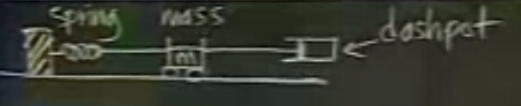
\includegraphics[height=2cm]{12_1.png}

Ortada duran kutle ileri geri gidebiliyordu, eger denklemde $f(t)$ varsa,
biri o kutle uzerinde ek olarak direk bir guc uygulamis olur, mesela
kutlenin bir metal oldugunu farzedelim, ve uzaktan birinin bir miknatis
tutarak yay, engelleyici ``haricinde'' degisik bir yonden de bir guc
uyguladigini hayal edelim. 

$f(t)=0$ oldugu zaman (yani denklemde olmadigi zaman), sistem
pasiftir. Disaridan hicbir guc uygulanmamaktadir. Baslangic sartlari olarak
bazi seyler yapabiliriz tabii, mesela kutleyi bir tarafa dogru cekip,
birakmak gibi. Ama ondan sonra sistemde hersey kendiliginden olacak, sistem
salinima girecek, ya da girmeyecek, vs. Eger $f(t)$ varsa, bu sisteme guc
uygulanmis sistem (forced system) denmesi bu yuzden. 

Ornek 2

Diferansiyel bir modeli mukemmel bir sekilde takip eden bir diger sistem,
basit bir elekrik devresidir.

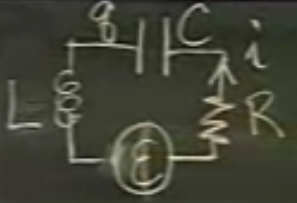
\includegraphics[height=2cm]{12_2.png}

$L$ bobinin yarattigi olusturucu (inductance) terimidir. Bu devreyi temsil
etmek icin iki diferansiyel denklem kullanilir, ama bu denklemlerden biri
otekinden turetilebilir, ikisi de Kirchoff'un voltaj kanununa baglidir. Bu
kanun der ki ``devrenin tum noktalarinda alinan voltaj farkliliklari /
dusuklukluklerini toplarsak, sonuc sifir olmalidir''. 

$q$ kapasitans uzerindeki akim (charge), $i$ devredeki akimdir. 

Denklem soyle

\[ Li' + Ri + \frac{q}{C} = \varepsilon(t) \]

Sagdaki $\varepsilon$ belki bir pil, bir jenerator uzerinden devreye
eklenen enerji. Bu enerji sinussel bir dalga seklinde olabilir, ki o zaman
alternatif akimdan (AC/DC) bahsediyor olurduk, ya da sabit olabilir, o
zaman duz akimdan (DC) bahsediyor olurduk. 

Formul hala nihai formunda degil, oraya gelmek icin bir sey daha bilmemiz
gerekiyor, $q' = i$, yani akimin kapasitoru terk edis hizi devrenin akima
esittir, akim bu yuzden hareket eder. Tabii aslinda hareket eden bir sey
yok, her elektron yanindakini ittirir, ama aslinda yerlerini terk etmezler,
her neyse [hoca ben de bu isi tam anlamiyorum diyor], her neyse, bu noktada
iki sey yapabiliriz. Ya tum denklemi entegre ederiz ve her seyi $q$ bazinda
temsil ederiz, ya da denlemin turevini aliriz ve her seyi $i$ bazinda
temsil ederiz. Bir turev yontemini takip edecegiz:

\[ Li'' + Ri' + \frac{i}{C} = \varepsilon(t)'\]

Eger sag tarafta duz akim olsaydi turev sonrasi $\varepsilon(t)'$'nin sifir
olacakti. Boylece elimize homojen bir denklem gecmis olurdu.

Eger duz akim bile koymamis olsaydik, yani devreye disaridan ek
yapmasaydik, belki baslangic sarti olarak kapasitor icinde bir doluluk
olabilirdi, ve bu akim yavasca devre uzerinden, az amartisorlu durumda
mesela ileri geriye bir salinimla, akacak ve bitecekti. Ama genellikle
uygulamalarda olan disaridan enerji verilmesi ve akimin ittirilmesi /
surulmesi / idare edilmesi, ve buna gore akimin ne olacaginin
hesaplanmasi. 

Elimizdeki iki problemler iste bunlar. Ya pasif devre, ya da disaridan
verilen enerji. 

Simdi homojen bir denklemi cozmek icin gereken kilit teoremi gorelim. 

Teori

\[ Ly = f(x) \]

Ustteki bir ODE ve $L$ bir lineer operator. O zaman cozum su formdadir:

\[ y_p + y_c \]

yani

\[ y = y_p + c_1y_1 + c_2y_2 \]

$y_p$ ozel (particular) cozum. Bu kelime bu dersin en kotu secilmis / kafa
karistirici kelimelerinden biri. Ozel cozum derken sanki ozgun, tekil
cagrisimi yapiliyor ama aslinda kastedilen herhangi bir cozum. 

Teoriye donelim, eger $L$'in lineer operator olusunu kullanirsak teorinin
ispati cok kolay. Iki ifadeyi ispatlamamiz gerekiyor. 

1. Tum $y = y_p + c_1y_1 + c_2y_2$ ifadeleri cozumdur. Bu ifadeyi nasil
ispatlariz? Ana denkleme koyarak. 

\[ L(y_p + c_1y_1 + c_2y_2) \]

Ustteki lineer operator olduguna gore

\[ = L(y_p) + L(c_1y_1 + c_2y_2) \]

Biliyoruz ki

\[ = \underbrace{L(y_p)}_{f(x)} + \underbrace{L(c_1y_1 + c_2y_2)}_{0} \]

\[ =f(x) \]

Demek ki tum $y_p + c_1y_1 + c_2y_2$'ler bir cozumdur. 

Bu hikayenin bir yarisi tabii. Hikayenin ikinci yarisi bu cozumlerin
``yegane'' cozumler oldugunu gostermek. Simdi ortaya $u(x)$ diye ufaklik
cikartacagiz, bu arkadas cozum oldugunu zannedecek. Ve bizde ispatta
gostermeliyiz ki bu kendini farkli zanneden $u(x)$ bile $y_p + c_1y_1 +
c_2y_2$ 
ifadesinden baska bir sey olamaz.

Bunu nasil yapacagiz. Cok kolay. Eger bir cozum ise 

\[ L(u) = f(x) \]

olmalidir. Peki su bizim ``ozel cozumu'' kullanalim, $L(y_p)$ nedir? Aynisi

\[ L(y_p) = f(x) \]

Son iki denklemi birbirinden cikartirsak

\[ L(u) - L(y_p) = 0 \]

\[ L(u - y_p) = 0\]

O zaman ustteki son ifade homojen denklemin bir cozumudur. O zaman su dogru
olmali

\[ u-y_p =  \tilde{c_1}y_1 + \tilde{c_2}y_2 \]

Diger yandan onceden bildigimiz gibi

\[ y = y_p + c_1y_1 + c_2y_2 \]

\[ y -  y_p = c_1y_1 + c_2y_2 \]

Ya da 

\[ u = y_p + \tilde{c_1}y_1 + \tilde{c_2}y_2 \]

\[ y = y_p + c_1y_1 + c_2y_2 \]

Son iki ifade birbirinin aynisi, o zaman $u$ farkli bir cozum olamaz. 

Eger katsayilar sabit ise, isin yarisini halletmisiz demek ki. Tamamlayici
denklemi biliyorsak, ki onu nasil bulacagimizi biliyoruz artik, ustel,
kompleks ustel, sin, cos fonksiyonlar kullanarak, vs. Geriye ne kaliyor?
Sadece ozel bir cozum bulmak kaliyor. Yani hangisi olursa olsun, esitligin
sag tarafina uyan ``bir'' cozum buldugumuz anda, isimiz bitiyor. 

Is bitiyor dedik ama, onumuzdeki iki haftayi bu ozel cozumu bulmakla
gecirecegiz. Fourier Serilerini kullanan bir genel metot gorecegiz, cunku
bu serileri islemek icin iyi bir bahane bu, fakat sunu da eklememiz
lazim. Birkac standart fonksiyon icin operatorler kullanaran genel bir
yontem var, tum diger ``standart olmayan'' durumlar icin seriler
kullaniliyor, ya da yaklasiksallama (approximation) kullaniliyor. Eger
bunlari hicbiri islemezse, en kotu durumda bilgisayara hesaplattiririz, ve
sayisal cevabi ozel cozum olarak kullaniriz. 

Simdi bu yaptiklarimizi 1. seviye denklemlerle irtibatlandirmak
istiyorum. Ders 8'den hatirlayalim:

\[ y' + ky = q(t) \]

Cozum icin entegre edici faktoru bulmustuk, carpmistik, vs. Cozum soyleydi

\[ y = e^{-kt} \int q(t)e^{kt}dt + ce^{-kt} \]

Ustteki formul 2. seviye denklemi cozmek icin gosterdigimiz paradigmaya
nasil baglantili? Ustteki denklemde artinin sagindaki terim tamamlayici
denklemin cozumu gibi durmuyor mu? 

\[ y = e^{-kt} \int q(t)e^{kt}dt + \underbrace{ce^{-kt}}_{y_c} \]

Bu mantikli cunku $ce^{-kt}$ alttaki homojen denklemin cozumu degil mi? 

\[ y' + ky = 0\]

Bunu hemen ilk bakista goruyoruz (dersin bu seviyesinde artik bunu aninda
soyleyebilmemiz lazim). 

O zaman ustteki cozumde $y_c$'den geri kalanlar da ozel cozum olurlar, 

\[ y = \underbrace{e^{-kt} \int q(t)e^{kt}dt}_{y_p} + \underbrace{ce^{-kt}}_{y_c} \]

Itiraz edenler olabilir, ama bu $y_p$ icinde tanimsiz bir entegral var,
ayrica hic sabit yok, vs. Eger entegralin tanimsizligi bizi rahatsiz
ediyorsa, onu tanimli hale getirmenin numarasini gormustuk, alt sinir icin
bir  sifir koyariz, uste $t$ koyariz, vs. Sabit konusuna gelince, entegre
edince ortaya bir sabit cikmayacak mi? 

Devam edelim. Ustteki cozum hakkinda bir yorum daha yapmistik, hatirlarsak,
$k>0$ ve $k<0$ sartlari oyle farkli iki sonuca yol aciyor, oyle farkli
fiziksel anlamlara sebep oluyor ki, aslinda ustteki ayni forma bagli
olmalarina ragmen, bu sartlarin tamamen farkli denklemler olarak
gorulmeleri gerektiginden bahsetmistik. 

$k>0$, ustteki cozumu $y_c$'nin gecici (transient) $y_p$'nin sabit konuma
(steady-state) donustugu bir durum ortaya cikiyordu. Bu durumda baslangic
sartlarinin tanimladigi $c$'nin ne oldugu onemli olmuyordu, cunku $c$'yi
iceren kisim ne olursa olsun sifira gidiyordu. 

$k<0$ olunca isler degisiyor tabii, o zaman ust paragraftaki analiz ise
yaramiyor. 

Simdi yapmak istedigim ustteki anlatimin 2. ve daha ust seviye
denklemlerdeki karsiligini bulmak. 2. seviyeyi anlamak yeterli aslinda, onu
anlarsak, daha ust seviye denklemlerde yapilacaklar tipatip ayni. 

\[ y'' + Ay' + By = f(t) \]






\end{document}
